\documentclass{standalone}
\usepackage{mathpazo}
\usepackage{tikz}
\usetikzlibrary{calc}
\usetikzlibrary{arrows}

\begin{document}

\def\wat#1#2#3{
\begin{scope}[shift={#1}]
  \node[draw, circle, radius = 0.5] (#2) at (0,0) {#3};
  \draw (#2.north) -- ++(0, 0.5) node[below left] {*}
  -| ($(#2.west) + (-.5,0)$) node[above right] {*}
  -- (#2.west);
\end{scope}
}

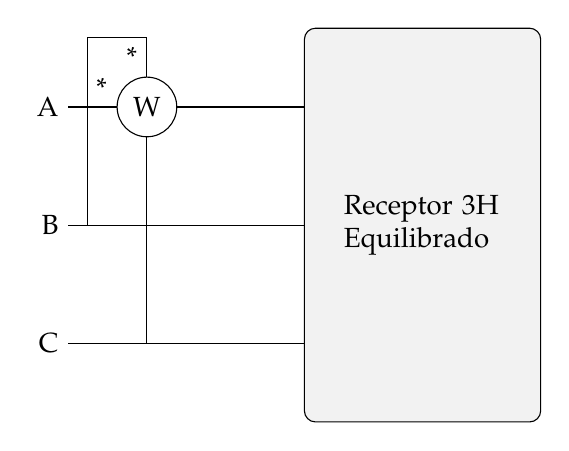
\begin{tikzpicture}
  %% Líneas
  \coordinate (A) at (-2,4.5);
  \coordinate (A') at ($(A) + (3, 0)$);
  \coordinate (B) at ($(A) + (0, -1.5)$);
  \coordinate (B') at ($(B) + (3,0)$);
  \coordinate (C) at ($(B) + (0, -1.5)$);
  \coordinate (C') at ($(C) + (3,0)$);
  %% vatímetro
  \node[draw, circle, radius = 0.5] (W) at ($(A) + (1, 0)$) {W};
  \draw (W.north) node[above left] {*};
  \draw (W.west) node[above left] {*};
  \draw (W.north) |- ++(-.75, 0.5)
  -- ($(B)!($(W.north) + (-.75,0)$)!(B')$);
  \draw (W.south)  -- ($(C)!(W.south)!(C')$);
  %% Salida de corriente de vatímetro
  \draw (W.east) -- (A');
  %% Entrada de corriente de vatímetros
  \draw (A) node[left] {A} -- (W.west);
  %% Linea A
  \draw (B) node[left] {B} -- (B');
  \draw (C) node[left] {C} -- (C');
  %% Salida de tensión de vatímetros
  %% Receptor
  \draw [rounded corners, fill= gray!10]
  ($(A') + (0, 1)$) rectangle ($(C') + (3,-1)$)
  node[midway, text width = 2cm] {Receptor 3H Equilibrado};
\end{tikzpicture}
\end{document}